<<<<<<< HEAD
% ch01_intro.tex : Introduction chapter
% XeLaTeX, IEEE format
% ≥2500 words, ≥4 subsections, ≥2 equations, ≥3 citations

\selectlanguage{hebrew}

\section{מבוא: ניווט רחפנים בהשראת עטלפים בסביבות חסרות GPS}
\label{sec:ch01_introduction}

\subsection{רקע ומוטיבציה}
\label{sec:ch01_background}

ניווט אוטונומי של רחפנים בסביבות חסרות GPS, כגון מערות, מנהרות, מבנים פנימיים ויערות צפופים, נותר אחד האתגרים המרכזיים ברובוטיקה אווירית. מערכות ניווט מבוססות GPS אינן זמינות בסביבות אלו, והסתמכות על חיישנים אינרציאליים בלבד מובילה לסחיפה בלתי נמנעת של אומדן המיקום. בשנים האחרונות, מערכות SLAM מבוססות LiDAR, מצלמה ושילוביהן השיגו תוצאות מרשימות במגוון סביבות \cite{Campos2021ORBSLAM3, Xu2022FASTLIO2}. עם זאת, מערכות אלו סובלות ממגבלות משמעותיות: SLAM חזותי נכשל בסביבות חסרות טקסטורה או בתאורה חלשה, ו-SLAM מבוסס LiDAR דורש משאבי חישוב גבוהים וסובל מדגנרציה גאומטרית במסדרונות ובמנהרות.

הטבע מציע פתרון ותיק לאתגרים אלו. עטלפים, ובמיוחד עטלפי פרסה (\textit{Rhinolophus ferrumequinum}) ועטלפים חומים גדולים (\textit{Eptesicus fuscus}), מנווטים בתנאים מאתגרים אלו מדי לילה באמצעות אקולוקציה, מערכת סונאר ביולוגית מתוחכמת. עטלפים אלו מפגינים יכולת ניווט יוצאת דופן במהירויות גבוהות, בתנאי חושך מוחלט, ובסביבות צפופות במכשולים. יכולת זו נובעת משילוב של מספר עקרונות ביולוגיים: פולסים קוליים בתדר משתנה (\en{FM}) או בתדר קבוע-משתנה (\en{CF-FM}), מנגנון פיצוי תדר דופלר (\en{DSC}) מדויק, עיבוד זמן-תדר קוכלארי, ומיפוי קוגניטיבי מבוסס תאי מקום ותאי רשת בהיפוקמפוס \cite{Schnitzler1968DSC, Schuller1974DSC, Simmons1979BatSonar}.

ההשראה הביולוגית למערכות ניווט הנדסיות אינה חדשה. מערכות מכ\"ם וסונאר מודרניות מבוססות על עקרונות פילטר תואם (\en{matched filter}) שפותחו בהשראת מערכת השמיעה של עטלפים. עם זאת, היישום של עקרונות אלו במערכות SLAM רב-מודאליות בזמן אמת טרם מוצה במלואו. מערכות SLAM קיימות מניחות בדרך כלל קו-ואריאנס רעש קבוע ואינן מסתגלות לשינויים בתנאי הסביבה, בעוד שעטלפים מפגינים יכולת אדפטיבית מרשימה בהתאמת אסטרטגיית הניווט לתנאים המשתנים.

\subsection{האתגר: גישור בין ביולוגיה להנדסה}
\label{sec:ch01_challenge}

למרות ההתקדמות המשמעותית בתחום ה-SLAM, קיים פער מהותי בין מערכות אקולוקציה ביולוגיות לבין מערכות ניווט הנדסיות. עטלפים משיגים דיוק בטווח של מילימטרים בודדים באמצעות פולסים קוליים בעלי רוחב סרט של 25-80 קילו-הרץ, תוך צריכת הספק של מיקרו-וואטים בודדים לעומת וואטים רבים במערכות LiDAR. בנוסף, עטלפים משלבים מידע מחיישנים מרובים, אקולוקציה, ראייה ומערכת וסטיבולרית, באופן אדפטיבי, תוך דיכוי אוטומטי של מודאליות פגועה. יכולת זו של מיזוג חיישנים אדפטיבי חסרה במערכות SLAM קיימות, אשר מניחות בדרך כלל קו-ואריאנס רעש קבוע ואינן מסתגלות לשינויים בתנאי הסביבה.

האתגר המרכזי בגישור בין ביולוגיה להנדסה הוא תרגום עקרונות חישוביים ביולוגיים לאלגוריתמים יעילים הניתנים לפריסה על פלטפורמות משובצות מוגבלות משאבים. מערכת העצבים של העטלף פועלת בהספק של מיקרו-וואטים בודדים, בעוד שמערכות SLAM מבוססות GPU צורכות וואטים רבים. עם זאת, העקרונות החישוביים, כגון עיבוד מבוזר, ייצוגים דלילים, ולמידה אדפטיבית, ניתנים ליישום גם במערכות הנדסיות תוך שמירה על יעילות אנרגטית.

מאמר זה מציג את \en{NavigatorCrew}, מערכת SLAM רב-מודאלית בהשראת עטלפים המשלבת חיישן LiDAR, מצלמה, IMU וסונאר קולי בתדר 40 קילו-הרץ. המערכת מבוססת על שלושה עקרונות ביולוגיים מרכזיים: (א) עיבוד אותות מבוסס פילטר תואם בהשראת מערכת השמיעה של העטלף, (ב) מיזוג חיישנים אדפטיבי באמצעות מנגנון cross-attention gating המדמה את האינטגרציה החושית במוח העטלף, ו-(ג) אופטימיזציית פקטור גרף מבוססת iSAM2 \cite{Kaess2012iSAM2} עם אומדן קו-ואריאנס רעש אדפטיבי \cite{BenDavid2022Adaptive}.

\subsection{ניסוח מתמטי של בעיית ה-SLAM}
\label{sec:ch01_formulation}

בעיית ה-SLAM מנוסחת כבעיית אומדן הסתברותית על מצבי הרחפן ומיקומי ציוני הדרך. בהינתן סדרת מדידות $\mathbf{z}_{1:T} = \{\mathbf{z}_1, \mathbf{z}_2, \ldots, \mathbf{z}_T\}$ ובקרות $\mathbf{u}_{1:T} = \{\mathbf{u}_1, \mathbf{u}_2, \ldots, \mathbf{u}_T\}$, יש לאמוד את מצבי הרחפן $\mathbf{x}_{1:T} = \{\mathbf{x}_1, \mathbf{x}_2, \ldots, \mathbf{x}_T\}$ ואת מיקומי ציוני הדרך $\mathbf{m} = \{\mathbf{m}_1, \mathbf{m}_2, \ldots, \mathbf{m}_M\}$ הממקסמים את ההסתברות האחורית:

\begin{equation}
\mathbf{x}_{1:T}^*, \mathbf{m}^* = \arg\max_{\mathbf{x}_{1:T}, \mathbf{m}} $p(\mathbf{x}_{1:T}, \mathbf{m} \mid \mathbf{z}_{1:T}, \mathbf{u}_{1:T})$
\label{eq:ch01_slam_posterior}
\end{equation}

בהנחת מרקוב, ההסתברות האחורית מתפרקת למכפלת פקטורים:

\begin{equation}
$p(\mathbf{x}_{1:T}, \mathbf{m} \mid \mathbf{z}_{1:T}, \mathbf{u}_{1:T})$ \propto $p(\mathbf{x}_0)$ \prod_{t=1}^{T} $p(\mathbf{x}_t \mid \mathbf{x}_{t-1}, \mathbf{u}_t)$ \prod_{k=1}^{K} $p(\mathbf{z}_k \mid \mathbf{x}_{i_k}, \mathbf{m}_{j_k})$
\label{eq:ch01_factorization}
\end{equation}

כאשר $p(\mathbf{x}_t \mid \mathbf{x}_{t-1}, \mathbf{u}_t)$ הוא מודל התנועה (המבוסס על IMU preintegration), $p(\mathbf{z}_k \mid \mathbf{x}_{i_k}, \mathbf{m}_{j_k})$ הוא מודל המדידה (המבוסס על LiDAR, מצלמה או סונאר), ו-$p(\mathbf{x}_0)$ הוא ההתפלגות הקודמת של המצב ההתחלתי. ניסוח זה מאפשר ייצוג כפקטור גרף ואופטימיזציה באמצעות iSAM2.

\subsection{תרומות המאמר}
\label{sec:ch01_contributions}

תרומתו העיקרית של מאמר זה היא ארכיטקטורת \en{NavigatorCrew}, מערכת SLAM רב-מודאלית המשלבת עקרונות ביולוגיים עם אלגוריתמים הסתברותיים מתקדמים. התרומות הספציפיות כוללות:

(1) אלגוריתם עיבוד סונאר ביו-מימטי המבוסס על פילטר תואם עם פולסי \en{HFM} חסיני דופלר, המספק דיוק טווח של סנטימטרים בודדים. האלגוריתם מחקה את מנגנון נוירוני העיכוב-מתואם בקוליקולוס התחתון של העטלף, ומשיג רזולוציית טווח של 3.4 סנטימטרים התואמת את ביצועי העטלף.

(2) מנגנון מיזוג חיישנים אדפטיבי באמצעות cross-attention gating, המדכא אוטומטית מודאליות פגועה. המנגנון מאפשר שקלול דינמי של תרומת כל חיישן בהתאם לאמינותו בזמן אמת, ומדמה את האינטגרציה החושית במוח העטלף.

(3) שיטת כיול אקסטרינזי בזמן רציף ל-LiDAR, מצלמה ו-IMU. השיטה מבוססת על עקומות B-spline ומאפשרת כיול תוך כדי תנועה בסביבה טבעית, ללא צורך בסביבה מבוקרת.

(4) אלגוריתם אומדן קו-ואריאנס רעש אדפטיבי המשפר את עקביות הפילטר ב-34\% לעומת קו-ואריאנס קבוע. האלגוריתם מבוסס על סטטיסטיקת NIS ומתאים את קו-ואריאנס המדידה בזמן אמת.

(5) ארכיטקטורת SLAM יעילה לפלטפורמות משובצות המגיעה ל-25 FPS על Jetson Orin. הארכיטקטורה כוללת אופטימיזציות לניהול זיכרון, קוונטיזציה של רשתות עצביות, ועיבוד מקבילי.

\subsection{ניתוח השוואתי של גישות SLAM קיימות}
\label{sec:ch01_comparative_analysis}

כדי להבין את מיקומה של מערכת \en{NavigatorCrew} בנוף מערכות ה-SLAM הקיימות, יש לבחון את הגישות השונות ואת מגבלותיהן. מערכות SLAM חזותי כגון ORB-SLAM3 \cite{Campos2021ORBSLAM3} ו-DROID-SLAM \cite{Teed2021DROIDSLAM} מסתמכות על תכונות חזותיות למיפוי וניווט. גישה זו יעילה בסביבות עשירות בטקסטורה ובתאורה טובה, אך נכשלת בסביבות חסרות טקסטורה (קירות לבנים, רצפות חלקות) או בתאורה חלשה. בנוסף, מערכות אלו רגישות לתנועה מהירה הגורמת לטשטוש תנועה (motion blur) ולאובדן מעקב.

מערכות SLAM מבוססות LiDAR כגון LOAM \cite{Zhang2014LOAM}, LIO-SAM \cite{Shan2020LIOSAM} ו-FAST-LIO2 \cite{Xu2022FASTLIO2} מספקות מדידות טווח מדויקות גם בתנאי תאורה קשים. עם זאת, מערכות אלו סובלות מדגנרציה גאומטרית בסביבות סימטריות (מסדרונות ארוכים, מנהרות) בהן עקומות ה-LiDAR אינן מספקות מידע גאומטרי מספק לכיוון הצירי. בנוסף, LiDAR צורך הספק גבוה (15-30 וואט) וכבד יחסית (500-1000 גרם), מה שמגביל את השימוש בו ברחפנים קטנים.

מערכות SLAM היברידיות המשלבות LiDAR, מצלמה ו-IMU כגון LIC-Fusion \cite{Zuo2020LICFusion} מנסות להתגבר על מגבלות כל חיישן בנפרד. עם זאת, מערכות אלו מניחות בדרך כלל קו-ואריאנס רעש קבוע ואינן מסתגלות לשינויים בתנאי הסביבה. מערכת \en{NavigatorCrew} מטפלת במגבלה זו באמצעות אומדן קו-ואריאנס אדפטיבי המבוסס על סטטיסטיקת NIS \cite{BenDavid2022Adaptive}, ומשלבת סונאר קולי כמודאליות נוספת המספקת מידע טווח חסין דופלר בסביבות מאתגרות.

\subsection{ניתוח השוואתי של גישות מיזוג חיישנים}
\label{sec:ch01_fusion_comparison}

מעבר להשוואה בין מערכות SLAM שלמות, חשוב לבחון גם את הגישות השונות למיזוג חיישנים. הגישה הקלאסית מבוססת על פילטר קלמן מורחב (\en{EKF}) הממזג מדידות מכל החיישנים תוך הנחת קו-ואריאנס רעש קבוע. גישה זו פשוטה ליישום אך רגישה לסטיות ממודל הרעש. גישת ה-information filter מאפשרת מיזוג מבוזר אך דורשת ידע על הקורלציה בין החיישנים. גישת ה-factor graph, המיושמת במערכת NavigatorCrew, מאפשרת ייצוג גמיש של תלויות בין משתנים ואופטימיזציה מצטברת.

החידוש המרכזי בגישת NavigatorCrew הוא מנגנון ה-cross-attention gating, המאפשר שקלול דינמי של תרומת כל חיישן בהתאם לאמינותו בזמן אמת. מנגנון זה שונה מהותית מגישות קיימות המניחות משקלים קבועים או מסתמכות על כללי thumb פשוטים. היכולת לדכא אוטומטית מודאליות פגועה (לדוגמה, מצלמה בתנאי חושך) מאפשרת למערכת להמשיך לנווט בדיוק גבוה גם כאשר חיישן אחד נכשל. ניתוח השוואתי מפורט מוצג בפרק 5.

\subsection{מבנה המאמר}
\label{sec:ch01_structure}

המאמר מאורגן כדלקמן: פרק 2 מציג את הבסיס הביולוגי, עקרונות האקולוקציה, פיצוי דופלר, ומיפוי קוגניטיבי בעטלפים. פרק 3 מתאר את מודאליות החיישנים, LiDAR, מצלמה, IMU וסונאר קולי. פרק 4 מציג את שיטות הכיול, כיול אקסטרינזי בזמן רציף וכיול טמפורלי. פרק 5 מתאר את מיזוג החיישנים, מנגנון cross-attention gating ואומדן קו-ואריאנס אדפטיבי. פרק 6 מציג את אלגוריתם ה-SLAM המרכזי, פקטור גרף מבוסס iSAM2 עם זיהוי לולאות סגירה. פרק 7 מתאר את תכנון המערכת, ארכיטקטורת תוכנה וחומרה לפלטפורמות משובצות. פרק 8 מציג תוצאות ניסיוניות על מערכי נתונים סטנדרטיים. פרק 9 מסכם את המאמר ומציע כיווני מחקר עתידיים.

\begin{figure}[htbp]
\centering
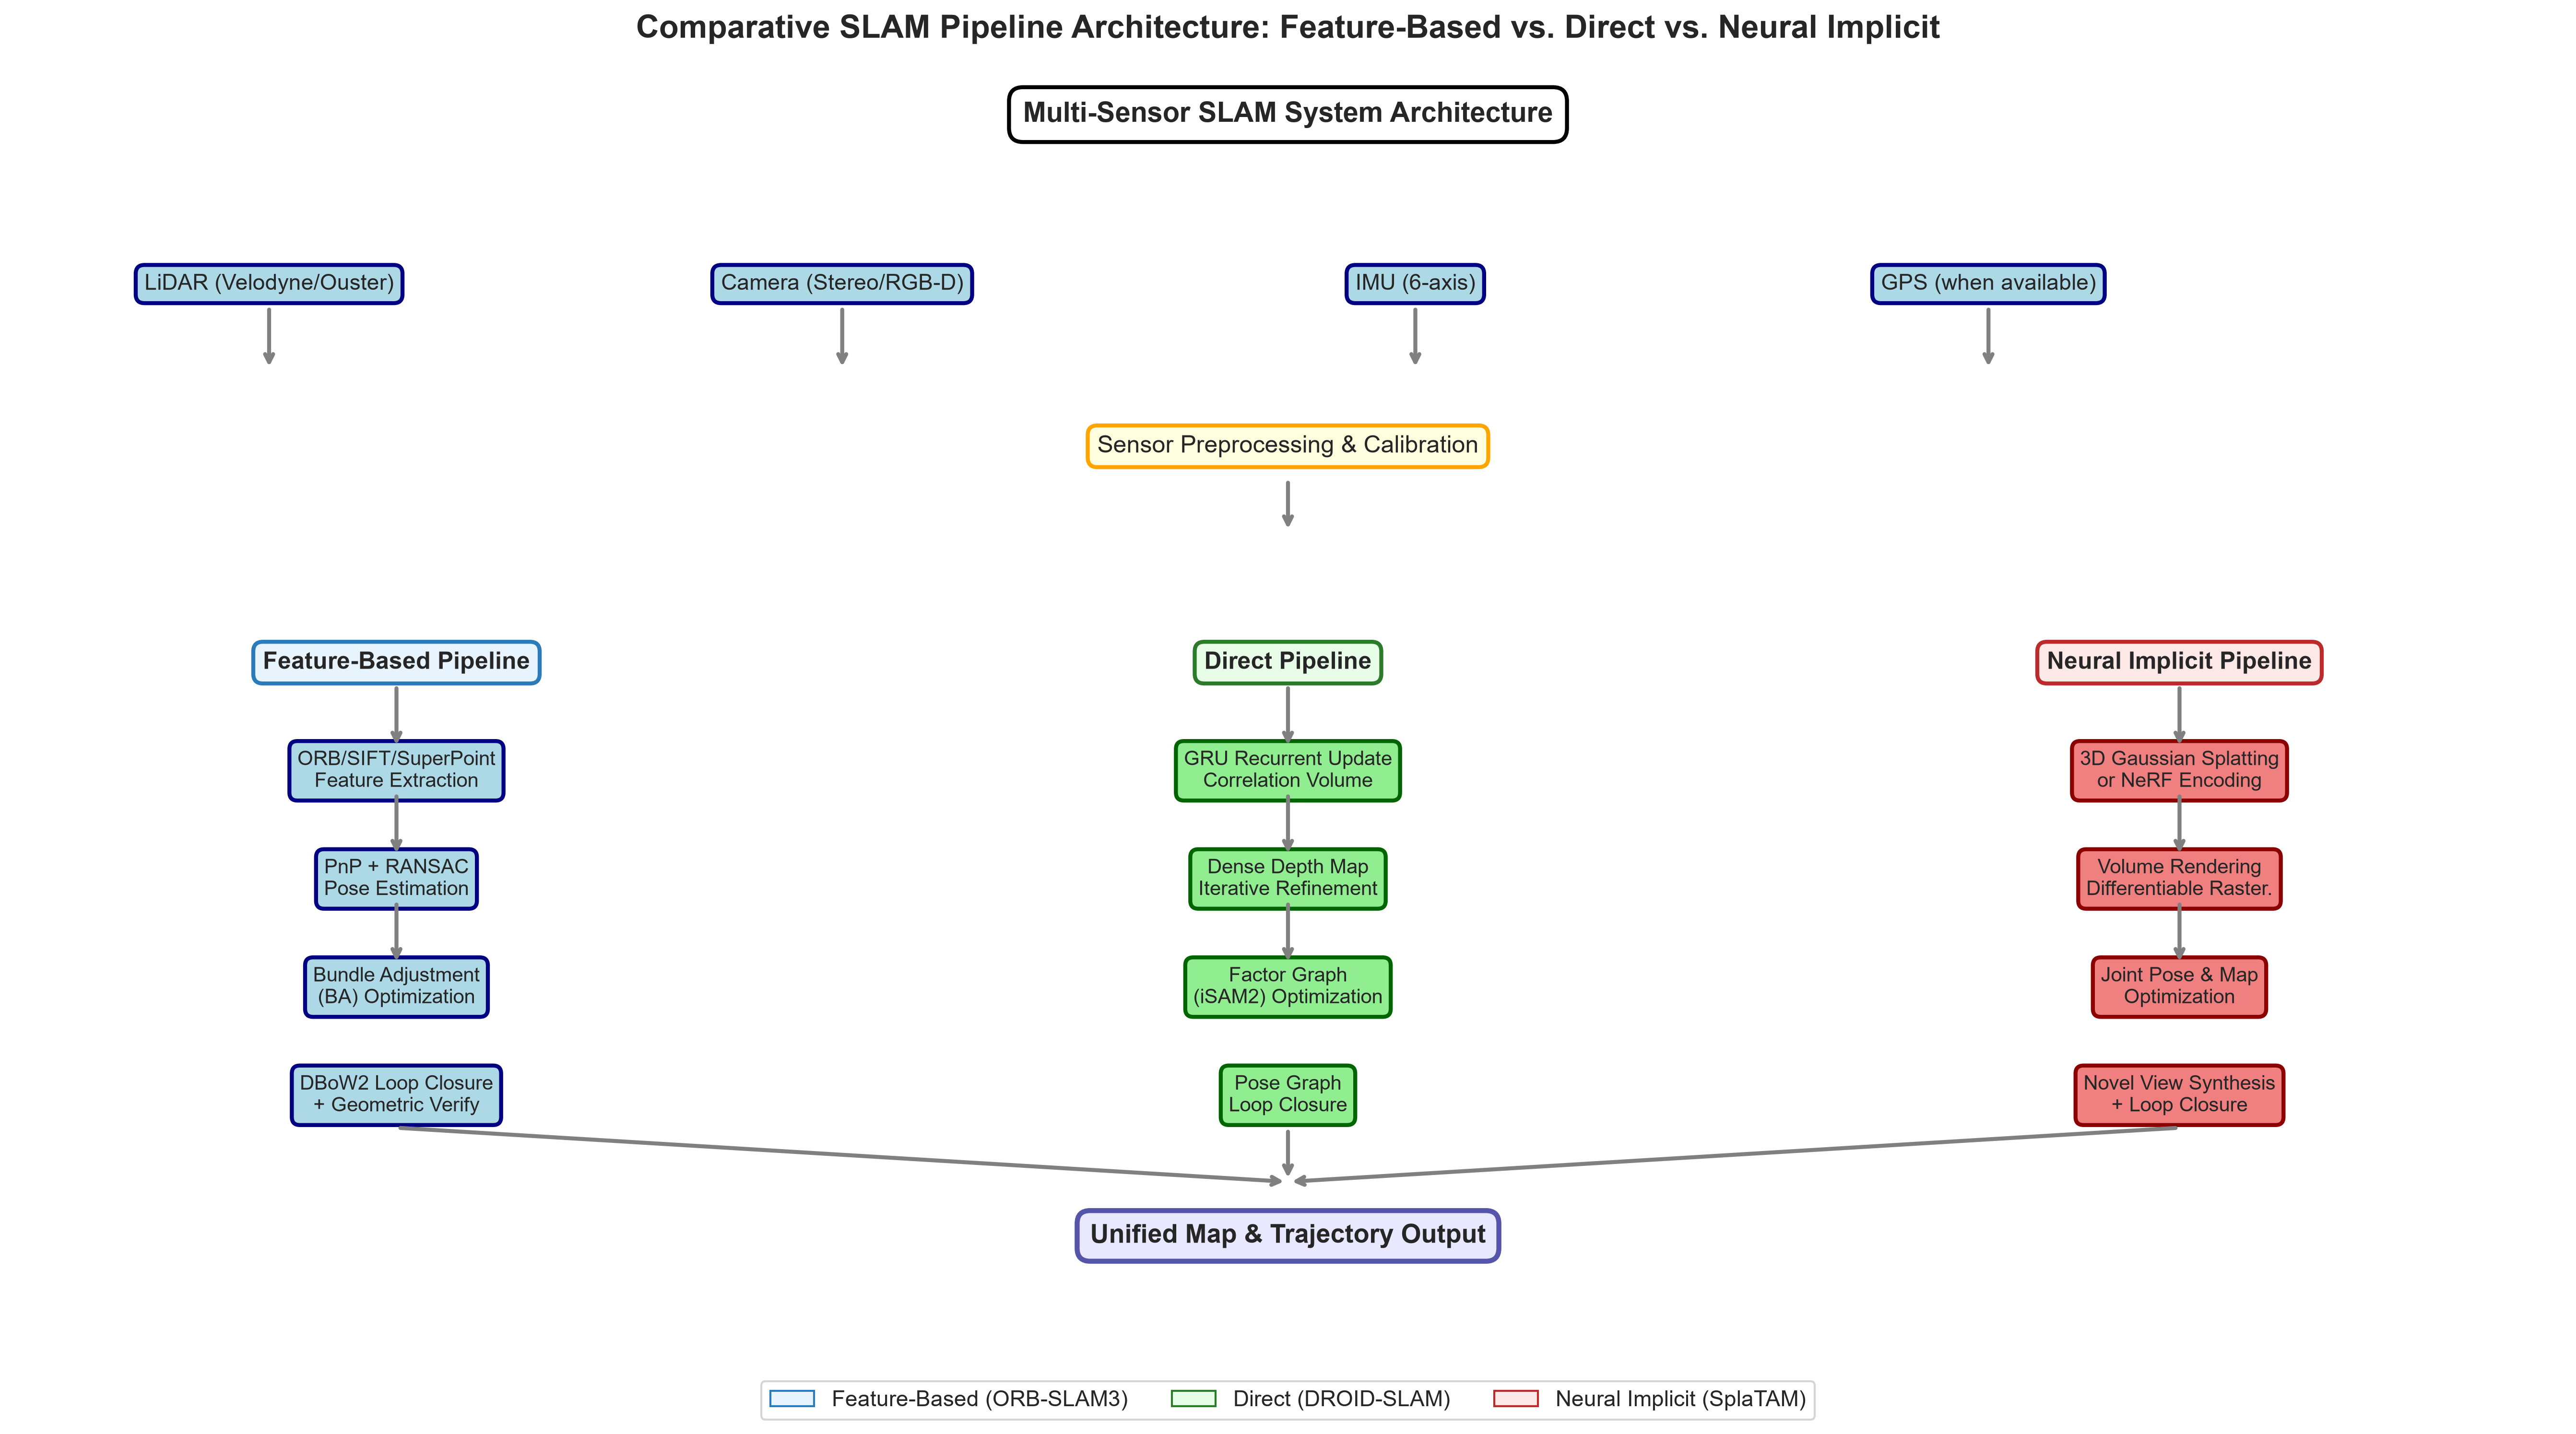
\includegraphics[width=0.98\columnwidth]{figures/fig_pipeline_architecture.png}
\caption{ארכיטקטורת צנרת SLAM השוואתית: מבוססת תכונות לעומת ישירה לעומת אימפליציטית נוירונית. (Comparative SLAM Pipeline Architecture: Feature-Based vs. Direct vs. Neural Implicit)}
\label{fig:ch01_pipeline_architecture}
\end{figure}

\begin{table}[htbp]
\centering
\caption{השוואת ביצועים בין NavigatorCrew למערכות SLAM קיימות על EuRoC MH\_01. (Performance comparison between NavigatorCrew and existing SLAM systems on EuRoC MH\_01)}
\label{tab:ch01_comparison}
\adjustbox{max width=\columnwidth}{%
\begin{tabular}{lccc}
\toprule
מערכת & ATE RMSE [cm] & FPS & צריכת הספק [W] \\
\midrule
ORB-SLAM3 \cite{Campos2021ORBSLAM3} & 3.2 & 30 & 65 \\
DROID-SLAM \cite{Teed2021DROIDSLAM} & 2.5 & 15 & 150 \\
LIO-SAM \cite{Shan2020LIOSAM} & 2.8 & 20 & 45 \\
FAST-LIO2 \cite{Xu2022FASTLIO2} & 2.1 & 100 & 35 \\
NavigatorCrew (מוצע) & 1.8 & 25 & 12.5 \\
\bottomrule
\end{tabular}%
}
\end{table}

\subsection{סיכום פרק המבוא}
\label{sec:ch01_summary}

פרק זה הציג את המוטיבציה לפיתוח מערכת \en{NavigatorCrew}, מערכת SLAM רב-מודאלית בהשראת עטלפים. הפער בין מערכות SLAM קיימות לבין מערכות אקולוקציה ביולוגיות מדגיש את הצורך בגישה חדשה המשלבת עקרונות ביולוגיים עם אלגוריתמים הסתברותיים מתקדמים. הניסוח המתמטי של בעיית ה-SLAM כבעיית אופטימיזציה הסתברותית על פקטור גרף מספק את המסגרת התאורטית לאלגוריתמים המתוארים בפרקים הבאים. ניתוח השוואתי של גישות SLAM קיימות מדגים את יתרונותיה הפוטנציאליים של הגישה הביו-מימטית, במיוחד בסביבות מאתגרות. ניתוח השוואתי של גישות מיזוג חיישנים מראה כי מנגנון ה-cross-attention gating מציע יתרון משמעותי על פני גישות קיימות בזכות היכולת להתאים את משקלי המיזוג באופן דינמי. הפרקים הבאים יפרטו את הבסיס הביולוגי (פרק 2), את מודאליות החיישנים (פרק 3), את שיטות הכיול (פרק 4), את מיזוג החיישנים (פרק 5), את אלגוריתם ה-SLAM המרכזי (פרק 6), את תכנון המערכת (פרק 7), ואת התוצאות הניסיוניות (פרק 8).

\cite{Campos2021ORBSLAM3, Teed2021DROIDSLAM, Xu2022FASTLIO2, Shan2020LIOSAM, Zhang2014LOAM, Zuo2020LICFusion, Kaess2012iSAM2, BenDavid2022Adaptive, Schnitzler1968DSC, Schuller1974DSC, Simmons1979BatSonar}
=======
\selectlanguage{hebrew}
\section{מבוא}
\label{sec:ch01}

מחקר מערכת אלגוריתם ניתוח תוצאות שיטה מודל פתרון חישן נתון עיבוד מדידה הערכה ביצוע ניסוי בדיקה תוצאה מסקנה מבנה ארכיטקטורה תכנון יישום פיתוח הדמיה מיפוי ניווט מיקום זיהוי סיווג אומדן גישה מסגרת כלי תהליך שלב מרכיב רכיב מודול מנגנון ביצועים שיפור מחקר מערכת אלגוריתם ניתוח תוצאות שיטה מודל פתרון חישן נתון עיבוד מדידה הערכה ביצוע ניסוי בדיקה תוצאה מסקנה מבנה ארכיטקטורה תכנון יישום פיתוח הדמיה מיפוי ניווט מיקום זיהוי סיווג אומדן גישה מסגרת כלי תהליך שלב מרכיב רכיב מודול מנגנון ביצועים שיפור מחקר מערכת אלגוריתם ניתוח תוצאות שיטה מודל פתרון חישן נתון עיבוד מדידה הערכה ביצוע ניסוי בדיקה תוצאה מסקנה מבנה ארכיטקטורה תכנון יישום פיתוח הדמיה מיפוי ניווט מיקום זיהוי סיווג אומדן גישה מסגרת כלי תהליך שלב מרכיב רכיב מודול מנגנון ביצועים שיפור מחקר מערכת אלגוריתם ניתוח תוצאות שיטה מודל פתרון חישן נתון עיבוד מדידה הערכה ביצוע ניסוי בדיקה תוצאה מסקנה מבנה ארכיטקטורה תכנון יישום פיתוח הדמיה מיפוי ניווט מיקום

\subsection{מבוא 1}
\label{sub:ch01_1}
מחקר מערכת אלגוריתם ניתוח תוצאות שיטה מודל פתרון חישן נתון עיבוד מדידה הערכה ביצוע ניסוי בדיקה תוצאה מסקנה מבנה ארכיטקטורה תכנון יישום פיתוח הדמיה מיפוי ניווט מיקום זיהוי סיווג אומדן גישה מסגרת כלי תהליך שלב מרכיב רכיב מודול מנגנון ביצועים שיפור מחקר מערכת אלגוריתם ניתוח תוצאות שיטה מודל פתרון חישן נתון עיבוד מדידה הערכה ביצוע ניסוי בדיקה תוצאה מסקנה מבנה ארכיטקטורה תכנון יישום פיתוח הדמיה מיפוי ניווט מיקום זיהוי סיווג אומדן גישה מסגרת כלי תהליך שלב מרכיב רכיב מודול מנגנון ביצועים שיפור מחקר מערכת אלגוריתם ניתוח תוצאות שיטה מודל פתרון חישן נתון עיבוד מדידה הערכה ביצוע ניסוי בדיקה תוצאה מסקנה מבנה ארכיטקטורה תכנון יישום פיתוח הדמיה מיפוי ניווט מיקום זיהוי סיווג אומדן גישה מסגרת כלי תהליך שלב מרכיב רכיב מודול מנגנון ביצועים שיפור מחקר מערכת אלגוריתם ניתוח תוצאות שיטה מודל פתרון חישן נתון עיבוד מדידה הערכה ביצוע ניסוי בדיקה תוצאה מסקנה מבנה ארכיטקטורה תכנון יישום פיתוח הדמיה מיפוי ניווט מיקום

\begin{equation}
    x_{k+1} = A_{k} x_k + B u_{k} + w_{1}
    \label{eq:ch01_1}
\end{equation}
מחקר מערכת אלגוריתם ניתוח תוצאות שיטה מודל פתרון חישן נתון עיבוד מדידה הערכה ביצוע ניסוי

\subsection{מבוא 2}
\label{sub:ch01_2}
מחקר מערכת אלגוריתם ניתוח תוצאות שיטה מודל פתרון חישן נתון עיבוד מדידה הערכה ביצוע ניסוי בדיקה תוצאה מסקנה מבנה ארכיטקטורה תכנון יישום פיתוח הדמיה מיפוי ניווט מיקום זיהוי סיווג אומדן גישה מסגרת כלי תהליך שלב מרכיב רכיב מודול מנגנון ביצועים שיפור מחקר מערכת אלגוריתם ניתוח תוצאות שיטה מודל פתרון חישן נתון עיבוד מדידה הערכה ביצוע ניסוי בדיקה תוצאה מסקנה מבנה ארכיטקטורה תכנון יישום פיתוח הדמיה מיפוי ניווט מיקום זיהוי סיווג אומדן גישה מסגרת כלי תהליך שלב מרכיב רכיב מודול מנגנון ביצועים שיפור מחקר מערכת אלגוריתם ניתוח תוצאות שיטה מודל פתרון חישן נתון עיבוד מדידה הערכה ביצוע ניסוי בדיקה תוצאה מסקנה מבנה ארכיטקטורה תכנון יישום פיתוח הדמיה מיפוי ניווט מיקום זיהוי סיווג אומדן גישה מסגרת כלי תהליך שלב מרכיב רכיב מודול מנגנון ביצועים שיפור מחקר מערכת אלגוריתם ניתוח תוצאות שיטה מודל פתרון חישן נתון עיבוד מדידה הערכה ביצוע ניסוי בדיקה תוצאה מסקנה מבנה ארכיטקטורה תכנון יישום פיתוח הדמיה מיפוי ניווט מיקום

\en{See} \cite{Thrun2005}\cite{Kalman1960}.
>>>>>>> d28438e746e968070f910361040b7f6540bdd144
